\documentclass[12pt]{article}

\usepackage[english]{babel}
\usepackage[a4paper, left=.8in, right=.8in, top=.5in, bottom=.5in]{geometry}
\usepackage{hyperref}
\usepackage[style=numeric,sorting=none,backend=bibtex]{biblatex}
\addbibresource{refs.bib}
\hypersetup{
	colorlinks=false,
	linkbordercolor={0 1 0},
	citebordercolor={1 0 0},
	urlbordercolor={0 0 1},
	pdfborderstyle={/S/U/W 1}
}
\usepackage{titling}
\usepackage{amsmath}
\usepackage{graphicx}
\usepackage{caption}
\usepackage{subcaption}
\usepackage{lmodern}
\usepackage[T1]{fontenc}
\predate{}
\postdate{}

\title{Visual Analytics for Underwater Super Resolution}
\author{Giovanni Ficarra}
\date{}

\begin{document}
	\maketitle

	\section{Introduction}\label{sec:intro}

	During my PhD, I am dealing with underwater image super resolution, that is ``the process of recovering high-resolution images from low-resolution images'' \cite{sr-survey}.
	In this field, the most used metrics to evaluate the performances of the proposed neural networks are SSIM (Structural SIMilarity) and PSNR (Peak Signal to Noise Ratio), but there is not a common agreement about their reliability. In fact, often a visual inspection shows that images with higher scores do not appear better than images with lower scores. Thus, it is hard to establish which are the best models.

	It is fundamental to find out which metrics are the most meaningful to proceed in the research of better SR models. To do this, it may be interesting to plot \textit{all} the results of our experiments and visually analyze the differences and similarities among them with respect to the scores they obtain according to the considered metrics.
	Moreover, it may be useful to check what images with analogous results across different experiments have and do not have in common, for example to build a more significant benchmark dataset.


	\section{Related Works}\label{sec:works}

	In the supplementary material \cite{galassounified} of \cite{galasso2013unified} by Galasso et al. (2013), the authors rely on \textit{scatter plots} to detect strange patterns in the results of neural networks for video segmentation: in each plot, a point is an image described by a pair of metrics (e.g. boundary precision-recall VS volume precision-recall). In this way, all the pairs of metrics are analyzed to discover when they agree and when they disagree, to find out if they are considering different but useful points of view or just making some errors.
	In particular, if a subset of images is aligned along one direction, but distant along the other, we can inspect those images to analyze the different behaviors of the two metrics and find a reason for their inconsistency, or discard one of the metrics.

	Our intent is to extend this approach with an interactive application which allows to select images from the scatter plots to easily compare them and exploit also other visualizations, such as a parallel coordinates plot and a box plot, to combine different insights.
	
	The code of this report and of the application is available on GitHub\footnote{\url{https://github.com/GioFic95/Visual-Analytics-for-Super-Resolution}}, while the web app is hosted on Heroku\footnote{\url{https://sheltered-taiga-09066.herokuapp.com/}}. Please note that, since it is hosted on a free server, it may be slow, especially when visualizing all the data.


	\section{Dataset and Libraries}\label{sec:dataset}

	For this project, we used a dataset composed of frames extracted from videos downloaded from Fish4Knowledge \cite{f4k}, Pexels\footnote{\url{https://www.pexels.com/it-it/}}, Nautilus Live\footnote{\url{https://nautiluslive.org/}}, and the website of the Ocean Exploration Video Portal of the National Centers for Environmental Information of the USA \cite{pacific}\footnote{\url{https://www.ncei.noaa.gov/access/ocean-exploration/video/}}.

	The resulting dataset was splitted in three parts, for training, validation and testing. Here will use the test set, composed of 960 images, together with their super-resolved counterparts, obtained through about fifty experiments, where we tried different compression methods and training datasets, and many model parameters.

	The dataset used for this project also includes, for each super-resolved image, its evaluation with SSIM, PSNR\_Y, PSNR\_RGB and LPIPS \cite{lpips}, already computed and stored in CSV files. Thus, the total amount of data is
	\begin{equation}
		960 \text{ images} \times 51 \text{ experiments} \times 4 \text{ metrics} = 195'840 \text{ values}.
	\end{equation}
	To better visualize such amount of data, our application allows to see only information relative to a subset of the dataset, based on which compression method and training dataset were used.

	This preprocessing was performed using Python libraries such as PyTorch, Pandas and Numpy, while the visualizations have been realized using Plotly\footnote{\url{https://plotly.com}, \url{https://plotly.com/python/}} and its Dash\footnote{\url{https://plotly.com/dash/}, \url{https://dash.plotly.com/}}.


	\section{Visualizations and Analytics}\label{sec:vis}

	Since our interest is in evaluating both metrics \textit{and} SR models, other visualizations with respect to the scatter plots proposed in \cite{galasso2013unified} can be useful too:
	\begin{itemize}
		\item \textbf{Parallel coordinates} plot with the average scores of each model, to show the performances of the networks according to the various metrics and compare them;
		\item Another \textbf{scatter plot} with two coordinates computed via \textbf{PCA}, to explore the possibility of finding new representative metrics, from the combination of the old ones;
		\item Pairs of original and super-resoluted \textbf{images}, shown when a point on a scatter plot is selected, to link the behavior of a model on that image with the score it obtained.
		\item A \textbf{box plot} with statistics of a selected subset of images, to analyze differences among the images across all the models.
	\end{itemize}

	\begin{figure}[h!]
		\centering
		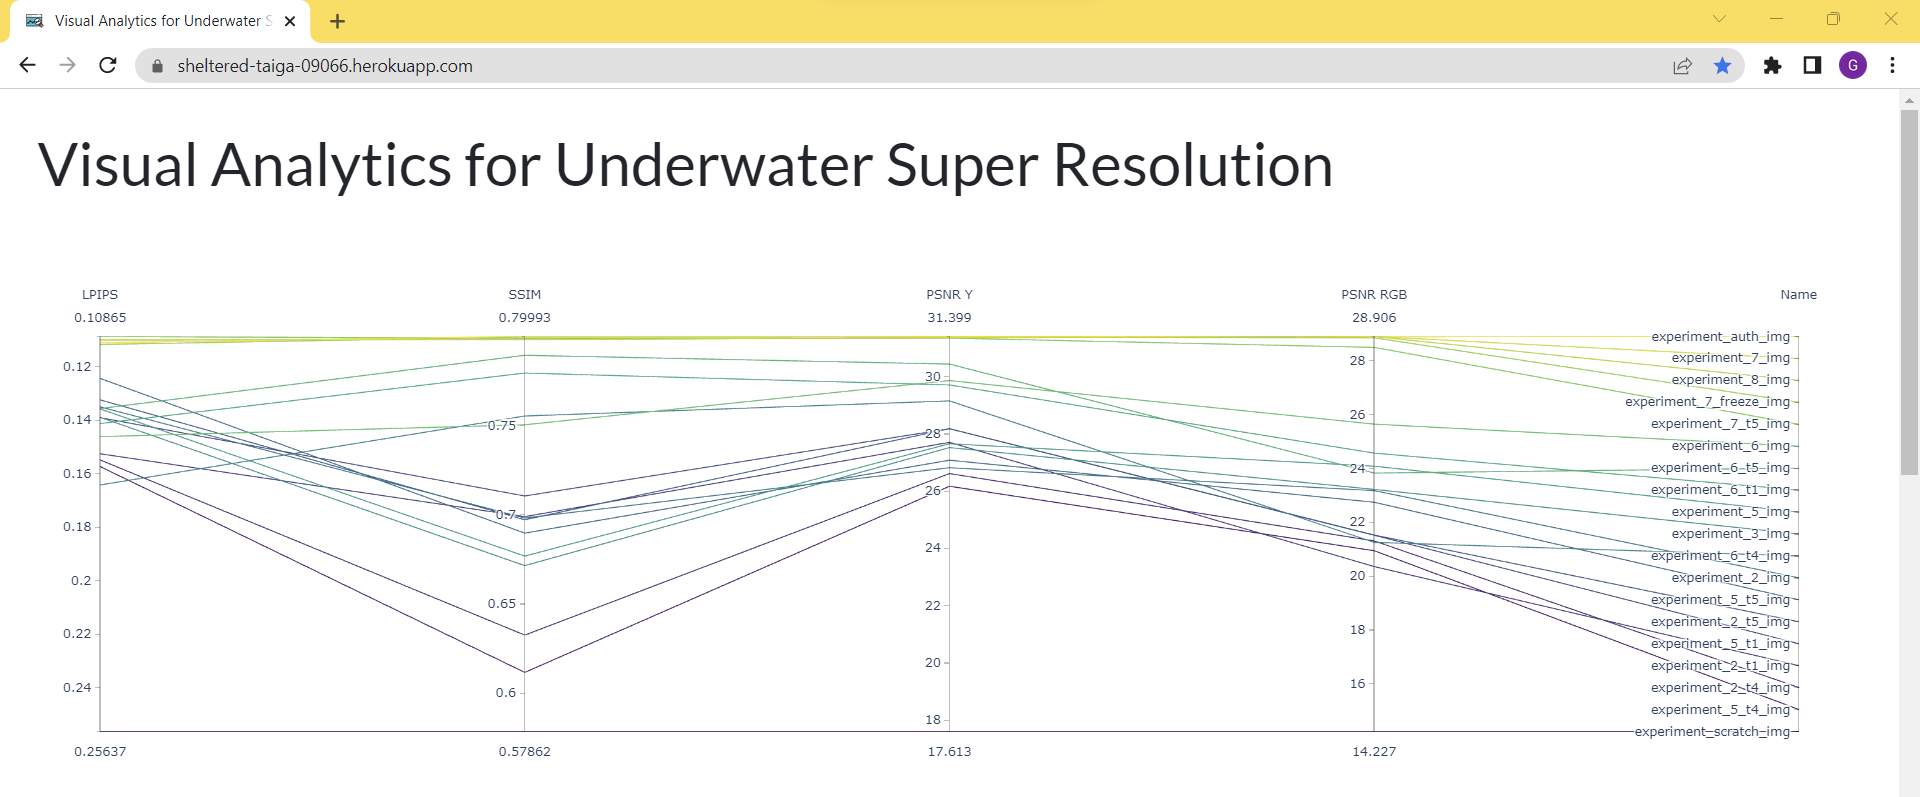
\includegraphics[width=0.7\linewidth]{imgs/parallel}
		\caption{The parallel coordinates plot}
		\label{fig:parallel}
	\end{figure}

	\subsection{The Parallel Coordinates Plot}\label{sec:parallel}

	The first part of the dashboard, in figure \ref{fig:parallel}, presents a parallel coordinates plot, which shows a set of experiments with their aggregated results, according to all the metrics. The models are dynamically ordered based on a composition of the metrics which takes into account which values are considered better for each metric (the higher the better or vice versa), i.e.:
	\begin{equation}
		\text{SSIM} + \text{PSNR\_Y} + \text{PSNR\_RGB} - \text{LPIPS}.
	\end{equation}
	In this way, the crossing among lines in the plot is minimized, since we have the best experiments at the top of it, and the worst at its bottom. Moreover, for the same reason, LPIPS, which resulted to be the most discordant metric, is by default at the first column of the plot.

	\textbf{Brushing} in the parallel coordinates plot allows to restrict the number of considered models also in the scatter plot.


	\begin{figure}[h!]
		\centering
		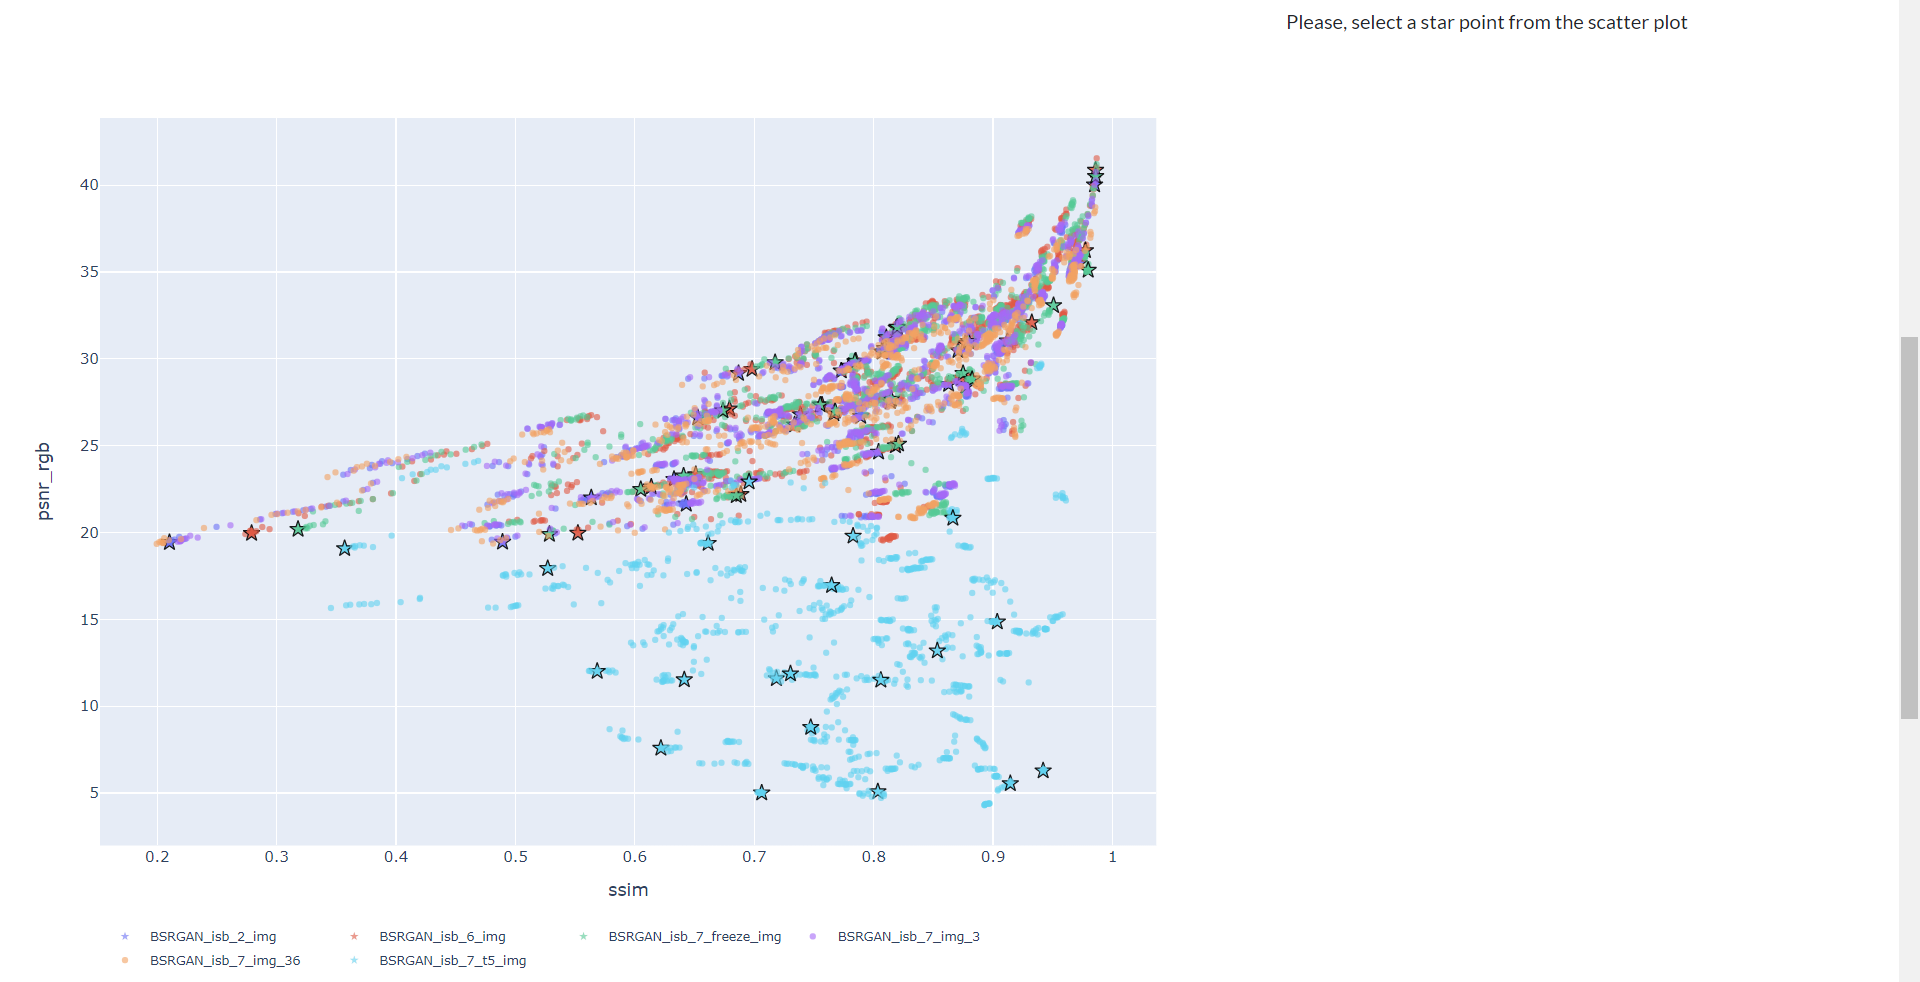
\includegraphics[width=0.7\linewidth]{imgs/scatter0}
		\caption{The scatter plot}
		\label{fig:scatter0}
	\end{figure}

	\subsection{The Scatter Plots}\label{sec:scatter}

	A set of scatter plots allows to compare pairs of metrics, to see if and when they agree and disagree. That is, each point in the plot is an image generated by a super-resolution model, with the coordinates given by two metrics selected by the user, and the color depending on the algorithm used to produce the image.

	A subset of the points is depicted as a \textbf{star}: in this way, we highlight some items to make it easier to select and compare them. In particular, most of these points are chosen such that they have similar value on one axis and different value on the other, that is, they are aligned along one of the axes, so that we can investigate on the images with maximum similarity according to one metric and dissimilarity according to the other.

	In the example in figure \ref{fig:scatters} we selected two images with very low PSNR\_RGB (\textasciitilde 5db) and quite high SSIM (\textasciitilde 80\% on the left, \textasciitilde 91\% on the right). We can clearly see that the second one, which should have higher quality, is not better than the first one.

	\begin{figure}[h!]
	\begin{subfigure}[H!]{0.5\textwidth}
		\centering
		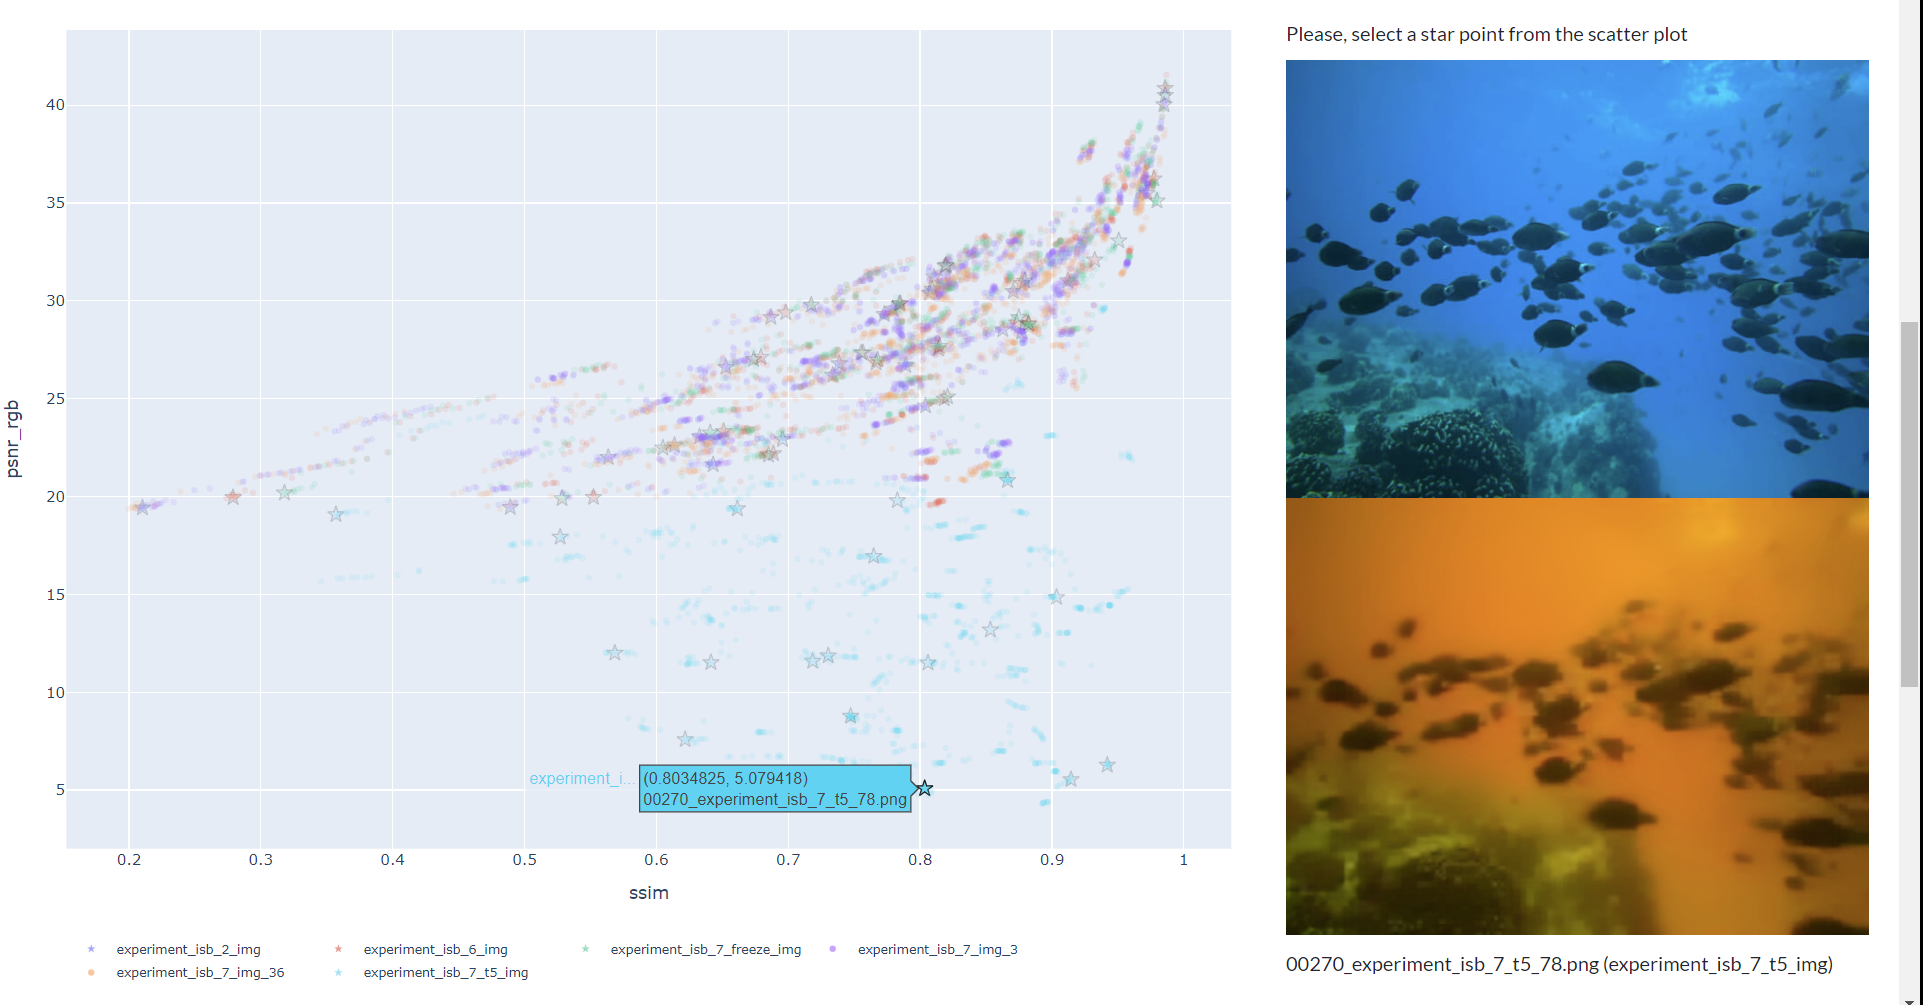
\includegraphics[width=0.9\linewidth]{imgs/scatter1}
		\label{fig:scatter1}
	\end{subfigure}
	\begin{subfigure}[H!]{0.5\textwidth}
		\centering
		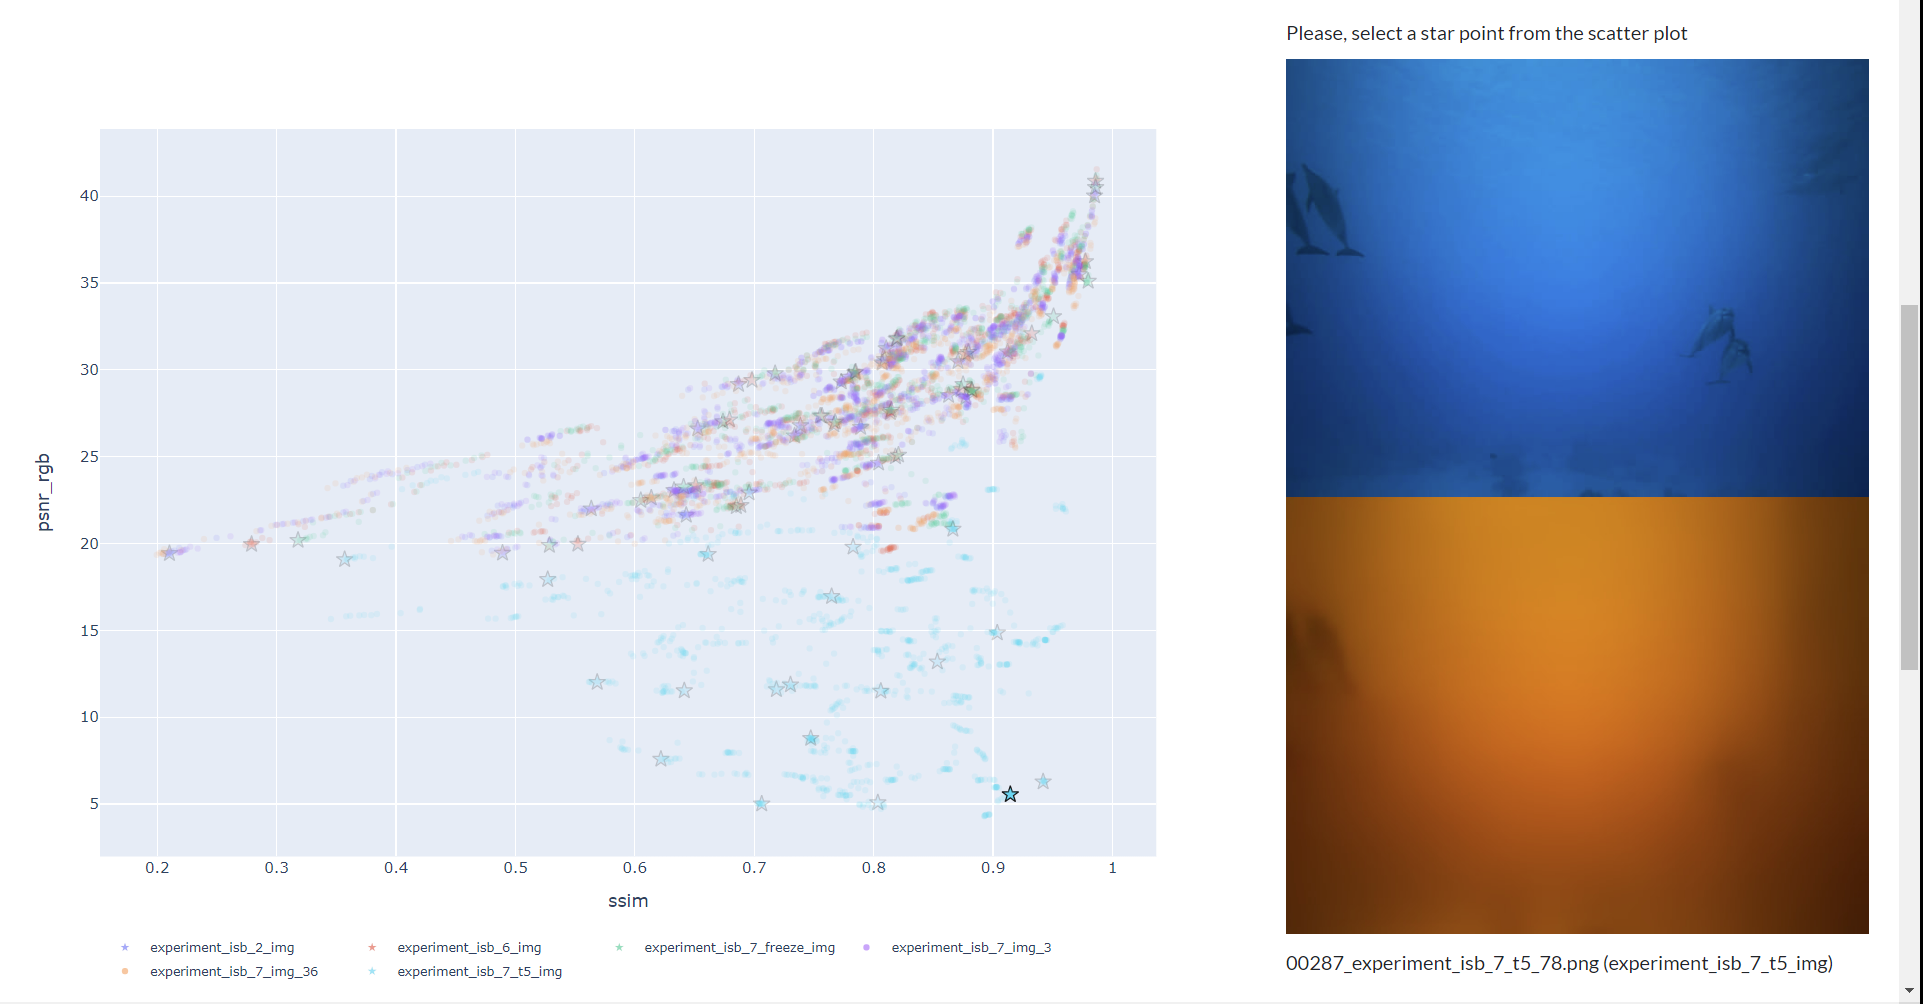
\includegraphics[width=0.9\linewidth]{imgs/scatter2}
		\label{fig:scatter2}
	\end{subfigure}
	\caption{The scatter plot with a selected image}
	\label{fig:scatters}
	\end{figure}

	The user can also choose to show the plot of the coordinates obtained with \textbf{PCA}. These values are computed when the application is launched, for the whole dataset, since the division into subsets is only intended for ease of visual consultation.

	The results seem to show that PCA\_X tends to put the best images on the left (negative values), while PCA\_Y puts them in the center (close to zero). These new metrics look more coherent with each other, in fact there is a small head on the left center of the plot and a large sparse tail on the right.

	\begin{figure}[h!]
		\centering
		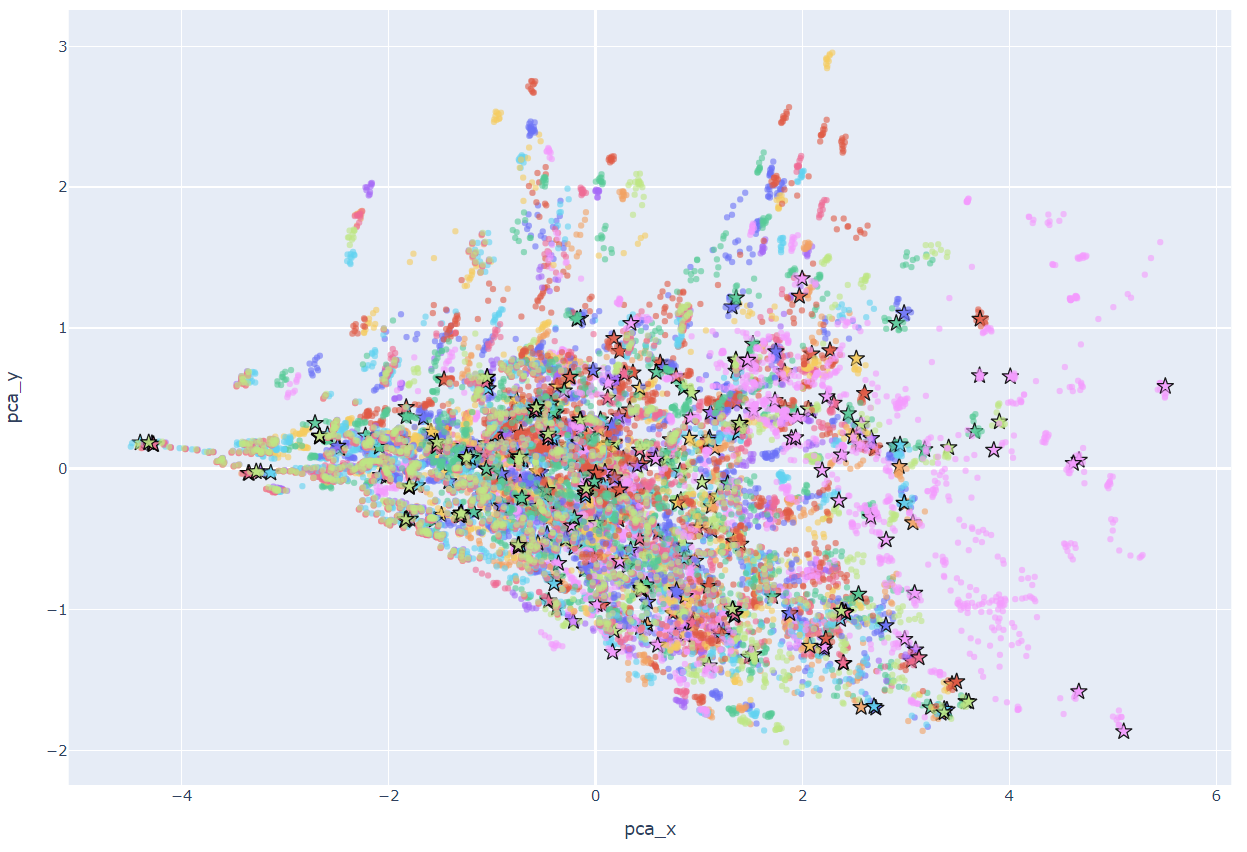
\includegraphics[width=0.6\linewidth]{imgs/scatter3}
		\caption{Scatter plot comparing PCA results}
		\label{fig:scatter3}
	\end{figure}


	\subsection{The Main Menu}\label{sec:menu}

	Between the parallel coordinates plot and the scatter plot there is the menu bar, composed of four elements:
	\begin{itemize}
		\item \textbf{Training dataset}: allows to select the dataset used to train the super-resolution model, between the training split of the one described in section \ref{sec:dataset} and the data provided to our group by a client of WSense\footnote{\url{https://wsense.it/}}, the company with which we are collaborating;
		\item \textbf{Compression type}: allows to select the compression type used to pre-process the images used as input for inference and testing;
		\item \textbf{Scatter metrics}: allows to select the pair of metrics to be compared in the scatter plot, including the coordinates produced by PCA;
		\item \textbf{Number of items}: shows the number of images in the dataset currently used to generate the parallel coordinates plot and the scatter plot.
	\end{itemize}

	\begin{figure}[h!]
		\centering
		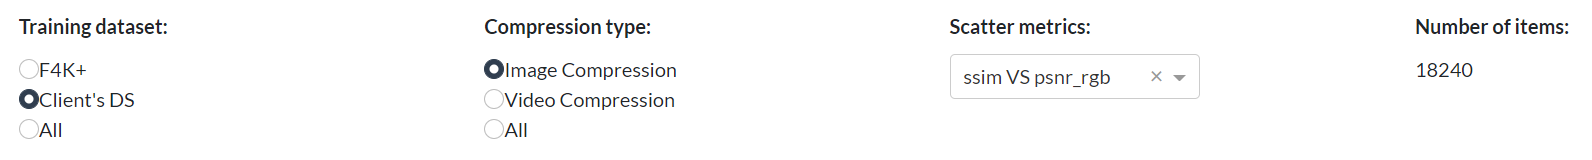
\includegraphics[width=0.7\linewidth]{imgs/menu}
		\caption{The main menu of the web app}
		\label{fig:menu}
	\end{figure}

	It is important to underline that the radio buttons affects the parallel coordinates plot, the scatter plot, and the box plot; the new selection reflects also on the counting of the items.

	The position of this menu makes it comfortable to click on the buttons both when looking at the parallel coordinates plot and at the scatter plot.


	\subsection{The Box Plot}\label{sec:box}
	
	A box plot is included to allow the user to further explore the dataset with respect to the general behavior of some images through all the considered experiments. In particular, when selecting a new subset through the main menu, the five elements with highest and lowest \textit{variance, standard deviation, mean, median, and difference between minimum and maximum} are computed and selected to be shown in the box plot.
	In this way, the user can click on any of these point and show the relative image, to study what pictures with similar and peculiar behaviors have in common, without overcrowding the plot with too many elements.
	
	A drop-down menu allows to select the metric based on which we want to further explore the dataset.

	\begin{figure}[h!]
		\centering
		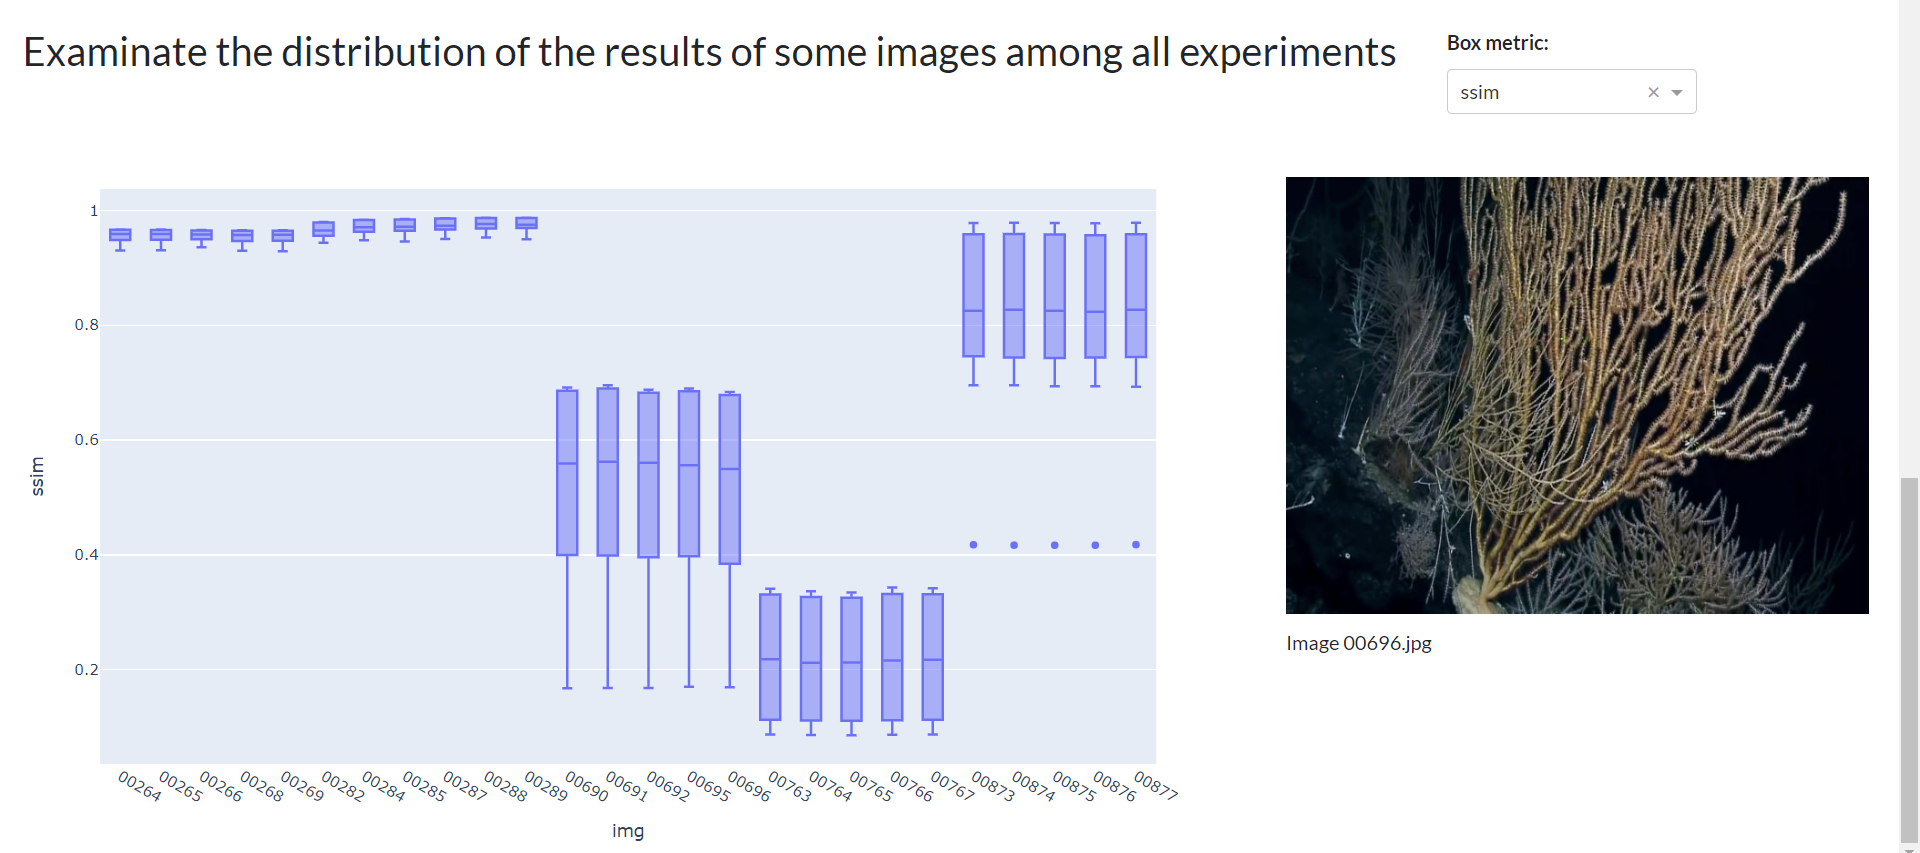
\includegraphics[width=0.7\linewidth]{imgs/box}
		\caption{The box plot}
		\label{fig:box}
	\end{figure}

	To enforce the idea that with the box plot we want to analyze the behavior of some images across all models, this diagram is kept separated from the others, thus also highlighting that filtering via brushing does not affect it.


	\section{Conclusion}\label{sec:conclusion}

	The implemented dashboard allows for an interactive visual inspection of the results of a set of experiments for underwater image super-resolution. The advantages of such analysis are various:
	\begin{itemize}
		\item Compare experiments at a glance;
		\item Easily compare images with respect to the scores they obtain;
		\item Find out which are the most reliable metrics;
		\item Define new metrics using PCA;
		\item Deeply explore a subset of significant images.
	\end{itemize}
	It may be interesting, in the future, to add the possibility to load any dataset, by just uploading pairs of original and super-resolved images, so that the same tool can be used by anyone with any image.
	Another feature worth including into the app would be the opportunity to add new metrics, from a list or even custom.


	\newpage
	\printbibliography
\end{document}
